\documentclass{article}
\usepackage{amsmath}
\usepackage{graphicx,xcolor}
\usepackage{wrapfig}
\usepackage[margin=1in]{geometry}
\usepackage[square,numbers]{natbib}
\bibliographystyle{unsrt}

\title{Information Extraction at the Edge with an Analysis Transaction and Value Ledger}
\author{Ryan Coffee}

\begin{document}

\maketitle

%\paragraph{Abstract:} %The advent of very high frame-rate sensors as needed for the upcoming ultra-high duty cycle user facilities in the Department of Energy research portfolio necessitates a fundamental shift in how experimental data is recorded and stored.
%A continued exponential increase in value from scientific experiments can only endure an impending end of Moore's scaling if we reinvent how experimental data is recorded, stored, reused, and compared with theory.
%An intelligent data pipeline is needed, one that is reconfigurable, robust, and reconstructable that incorporates machine learning and enables autonomous real-time decision making.
%Ideally this data pipeline would not only produce unique data identifiers but also would incentivize information sharing in an open data marketplace.


%\paragraph{Kelly notes:}
%Define a large problem that is viewed as important.
%Then give a credible list of milestones that deliver us some way toward the solution to that problem.
%BlockChain
%FPGA development (1st interaction with the data)
%GPU, TPU, FractalCore or other AI chip for the high-dimensional convolutions, RNN, or other initial layers
%Then different hardware, again maybe the Xilinx Veral chips for deeper fullyconnected.
%Then out through again FPGA, or direct to memory, or reverse back out for autoencoder.
%Decision output flags along the way.


%\paragraph{Send to Jana, Mike D, Chi-Chang\ldots and then to Daniel, Ian Foster (maybe), possibly someone from DANSS}


\section*{Executive Summary}
\paragraph{Problem Statement}% and Current state of the art}
\begin{wrapfigure}[33]{r}{.4\linewidth}
	\centerline{ 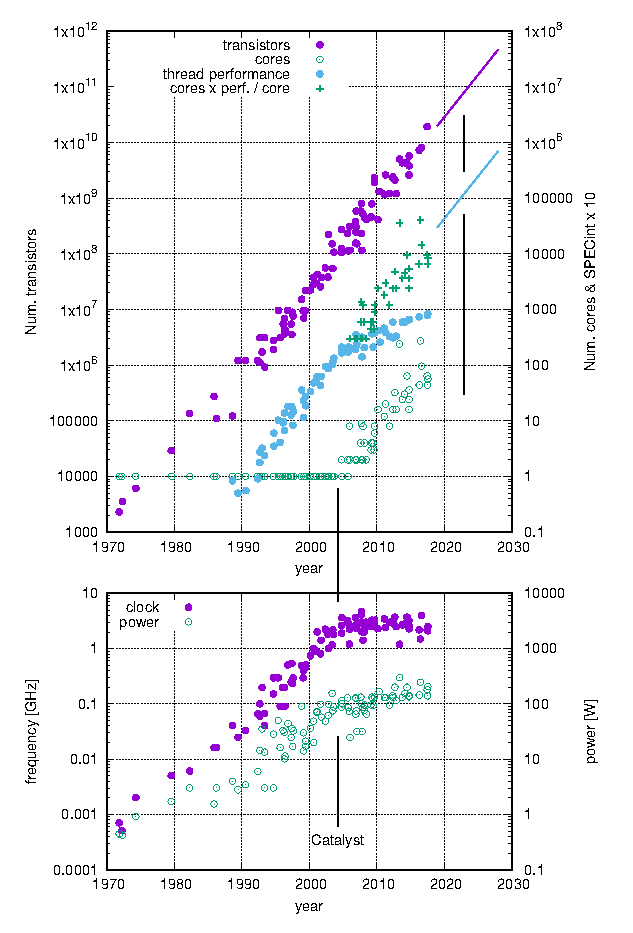
\includegraphics[clip,trim={-2cm -2cm 1.5cm 1.5cm},width=\linewidth]{plotting_technology.eps} }
	\caption{
		\label{fig::technology} 
		Data adapted from Ref.~\cite{MicroprocessorTrendData}. The mid-2000s saw that clock and thermal limitations (lower) triggered the multi-threading paradigm.
		Continued exponential growth in transistor density (upper, \textcolor{purple}{$\bullet$}) was matched with the multi-threading efficiency (upper, \textcolor{cyan}{$\bullet$} $\rightarrow$ \textcolor{green}{+}).
	}
\end{wrapfigure}
Processing data at the point of generation, at the sensor or cluster of sensors, is key to the future of Industrial Internet of Things (IIoT) \cite{Gartner2018,NetworkWorld2019}, also referred to as Industry 4.0.
In industry as in basic science, human technological advancement progresses with exponential rapidity \cite{Kurzweil}.
Particular to DOE's flagship facilities, data rates are growing to velocities of 100s of GB/s to TB/s that will quickly exceed network and storage capacity, thus providing early insight into the next decade of IIoT challenges.
We have an immediate need to reformulate data acquisition (DAQ) to the concept of information acquisition (IAQ)---we wish to record actionable information, not raw data, and to do it in a form that is flexible and compatible with the domain specific output targets.

Scientific advancement, like all human technological advancement, progresses with exponential rapidity \cite{Kurzweil} and in spite of physical limitations.
We see in the upper panel of Fig.~\ref{fig::technology} the increasing transistor density (upper: \textcolor{purple}{$\bullet$}).
When we hit the physical limitation of a few GHz (lower: \textcolor{purple}{$\bullet$}), industry immediately responded with the multi-threading paradigm (upper: \textcolor{green}{$\circ$}).
Physical limits are always circumvented by human creativity.
The computing bottleneck of this decade is now data transfer.
Our response to this limitation is already being formulated as Edge Computing \cite{thetech,NetworkWorld2019b}.
Much like multi-threading allowed continued exponential growth in the data center, Edge Computing will enable continued exponential growth of distributed sensors for autonomous decision making and information compression.

Although the Edge Computing paradigm has already begun, there is a rising concern for data security and provenance tracking \cite{brookings2019}.
Security that data is not being manipulated ``in-flight'' is certainly critical to autonomous vehicles, but one can also imagine how bad actors might mettle with or inject obfuscation into shared scientific data sets.
This would potentially harm the inferred results of data analysis and potentially mislead technological development.
Heading off such a threat by baking data provenance and verification directly into the adaptive Edge Computing paradigm is the route we propose to demonstrate, initially with a few crisp examples from DOE's user facilities, and then with expanded application to the broader industrial and health sector use cases.

\paragraph{Proposed solution}
Blockchain is a form of Distributed Ledger that is opening a new paradigm for data movement with collaborative verification and storage of transactional data.
We will initially focus on field programmable gate arrays (FPGAs) at the sensor to enable domain specific information extraction at the sensor that also initiates a unique ledger that recordes the analysis transactions used to extract, transform, and infer action from the data.
We will quickly include emerging Edge Computing microchips such as the EdgeTPU \cite{edgetpu_benchmarks,edgetpu}, coarse-grained reconfigurable arrays \cite{waveCGRA,CGRAreview}, ``sea-of-cores'' \cite{seaofcores} and others.
The chips will simultaneously execute the Edge inference models while updating the ledger.
The transaction chain will bind the fingerprint of the active model to the produced information in a uniquely identifiable provenance record as depicted in Fig.~\ref{fig::EdgeFlow}.
Encryption that uses this transaction ledger as the encryption ``salt'' will therefore require matching a valid ledger with its valid data set to achieve decryption.
The ledger record furthermore allows for dynamic data retention whereby lifetime in archive can scale with the scientific or social value derived from the data and/or algorithm.
value aggregation could then reveal the integrated value for scientific facilities or sensor technologies.

\begin{figure}
	\centerline{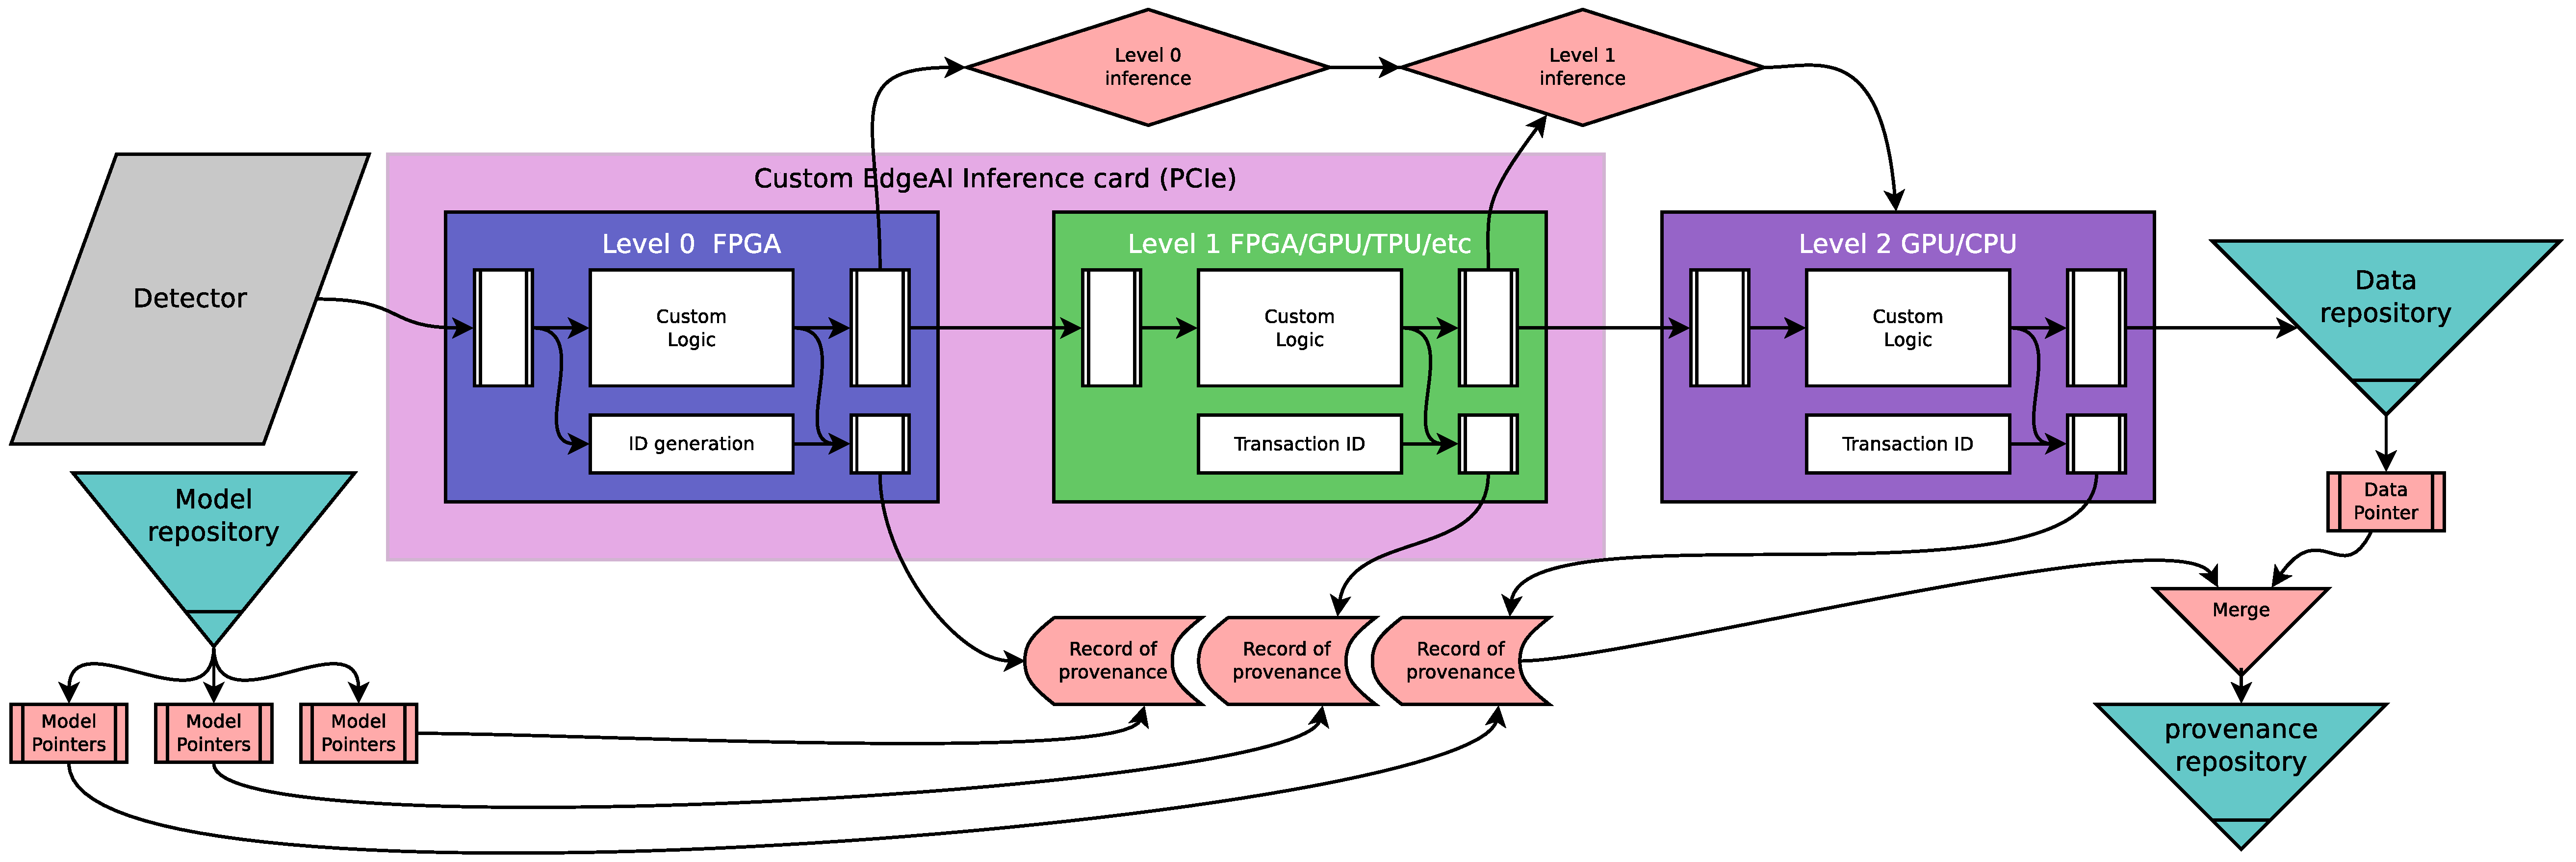
\includegraphics[clip,width=.75\linewidth]{EdgeFlow.eps}}
	\caption{
		\label{fig::EdgeFlow}
		Schematic of information flow through heterogeneous hardware with ID generation and provenance tracking.
		}
\end{figure}

\paragraph{Plan/Milestones}
%\emph{Year 1: \$750k + 50K for MHz camera + 20K in framegrabbers + 4x 120K digitizers}
In the first period we will concentrate on FPGA development for interpreting electron time of flight spectra for one of DOE's quintessential examples of a fire hose data source, the so-called CookieBox detector for LCLS-II.
We will demonstrate multiple pre-analysis algorithms in firmware of the digitizer FPGA where each algorithm is developed for a specific application of the detector.
These are unique domain specific algorithms that each effectively re-brand the detector for fundamentally different interpretations of the recorded analog waveforms.
This is why we concentrate initially on FPGAs for the sake of an expected weekly overhaul of the FPGA firmware.
We will demonstrate that the FPGA can generate the unique id that also binds to the corresponding algorithm, both of which yield a fingerprint to a unique data identifier.
This identifier will form the initial block in the transaction chain, thus initiating the hyper-ledger record.
The deeper analysis in subsequent AI acceleration chips that follow will then be treated as subsequent transactions that will be added to the ledger.

%\emph{Year 2: \$1M}
Following this initial demonstration, we will work together with the high frame rate camera producer and the associated frame-grabber supplier to demonstrate the same transaction ledger Edge Computing paradigm for image transformation.
The pre-analysis for images os often called ``featurization'' since it reduces typically MPix images into a more appropriate set of features before presenting to a machine learning inference model.
The featurization will occur in custom logic blocks in the frame-grabber FPGAs and then transfer directly to a more ML tailored inference chip such as a secondary inference accelerator \cite{waveCGRA,CGRAreview,seaofcores}.
In this case we will demonstrate tight coupling between the compiled byte-code and the generating code for the ML model along with identification of the training data pool used to produce the inference model.
These too will be treated as transactions that will be added to the blockchain.
At this stage we will also demonstrate the value-binding for data such that the beneficial outcome of the data and inference models can proportionately increment the ``retention value'' of the data element.
Also in this second phase we will explore an RF analog ASIC that includes the 16 channel ADC with the pre-analysis FPGA and downstream inference chip on a custom board.
This will allow for the full inference from all 16 data channels of the CookieBox to occur in an embedded inference engine that bypasses the PCIe bus.

%\emph{Year 3: \$1M }
In Year 3 we will work together with a high frame rate camera maker and the various AI acceleration chip makers to integrate what had previously been hosted on the frame-grabber into the camera electronics.
We will also help to define an daughter card integration standard to promote a unifying embedded EdgeAI for scientific as well as industrial and medical diagnostic sensors.
We attempt to intercept data and make modifications ``in-flight'' to show how it would render the data useless, spoiling the decryption algorithm.

\paragraph{Broader applications}
With an increasing reliance on machine learning for radio imaging applications in nuclear security comes the risk that such models can be nefariously altered.
This alteration can come from tampering with the models themselves or by injecting falsified training data into the training pool.
The ledger record will record interactions with the data in the training set such that attempts to use or alter the data will also appear in the transaction record.
Since the transaction record and training set fingerprints are used as so-called ``salt'' in the data encryption process, making it all but impossible to decrypt altered data.
Beyond nuclear security, the sharing of anonymized health data can be more securely controlled and therefore more confidently shared with exclusive trusted partners.
In the same way as the scientific data is itself imbued with follow-on value, so too with medical data; the originator of data could receive direct benefit for sharing, a benefit that could scale in proportion to the market value of output that derived from their data.
We note that the medical sensor portfolio is tremendous, it could even extend application to secure transfer and value tracking of in-home sensors for e.g. in-home elder care, nutrition, and diabetes.
%Smart connected in-home sensors with guarnateed privacy would facilitate elders to age in place, retaining thier physical social community.

\paragraph{Deliverables}
\begin{itemize}
	\item Domain specific interpretation of raw data via Edge Computing in multiple format sensor FPGAs, e.g. waveform digitizers and high frame rate imaging sensors.
	\item ASIC ID and FPGA firmware fingerprint used for unique identification and seed for data encryption.
	\item Transaction ledger based on block chain and distributed ledger technology that includes CPU model and code and GPU instructions as fingerprints written into the transaction record.
	\item Imbue original data with value that scales with the successful output from subsequent data transactions.
	\item Demonstrate that modifying data individuals in a training set renders the data useless and fundamentally spoils training convergence and identifies the offending transaction.
\end{itemize}

\bibliography{whitepaper.bib}

\break
\end{document}

\section{SUPPLIMENTAL}

\section{Motivation}

\subsection{Information not data}
\paragraph{Exponential advancement}
Scientific advancement, like all human technological advancement, progresses with exponential rapidity \cite{Kurzweil}.
At DOE's flagship facilities, data rates are likewise growing to velocities of 100s of GB/s to TB/s that will quickly exceed network and storage capacity.  
This challenge is not unique to the DOE, in a recent conversation with a leader in AI assisted agriculture it was noted that available hyperspectral imaging technology can not be appropriately used simply due to its excessive data velocity.
This is the concern of the upcoming light source facilities, the very high brightness beans and extreme pulse repetition rates will enable information acquisition but dectors and sensors will be unable to keep abreast of the data rate. 
Here, we key in on the idea of information acquisition, not data \textit{per se}, but actionable information in a form compatible with the user specific scientific targets being addressed by experiments.


\paragraph{Impending phase transition}
We see in the upper panel of Fig.~\ref{fig::technology} the increasing compute via the increasing transistor density.
There is as yet no indication of a physical limit in transistor number (purple filled circles), whereas we do see that the per-thread performance experienced a limit in the mid-2000s (blue filled circles).
In the lower panel, we explore this performace phase change via the clock rate and the power consumption.
The speed of light is 30 cm/ns such that the typical chip scale of 3 cm corresponds to one wavelength of 10 GHz light.
It is no suprise that, respecting Nyquist waveform sampling, we hit a physical clock limitation in the vicinity of a few GHz (purple filled circles).
As for power consuption and dissipation, the thermal conductivity of liquid water is on the order of $k \sim 7 $mW/cm/K.
We find a heat conductance of $q = k \delta T / \delta x \sim 3.5$ W/cm$^2$ for typical parameters and a typical 80cm$^2$ heat exchange area provides about 280W of cooling, also in appearant agreement with the power trend (green open cirles).
%\mbox{cm}^{-2}$ assuming $\delta T \simeq 50 \mbox{K}$ and $\delta x \simeq 0.1 \mbox{cm}$ is about 3.5 $\mbox{W} \mbox{cm}^{-2}$.
%For a heatsink of about $2\mbox{cm}\times2\mbox{cm}$ with 2 cm tall vanes separated by 1 mm gives a total surface area of about $80 \mbox{cm}^{2}$ and thus corresponds to a thermal dissipation capacity of 280 W.
%We note that the in the bottom panel of Fig.~\ref{fig::technology} we see that the power of the processors looks to be approaching a few hundred Watt assymptote.
At the time when technology hit these physical limitaitons, the industry nearly immediately responded with multi-threading (green open circles, upper panel).
When we account for this multi-threading by scaleing the per-thread performance by the number of threads (blue triangles) we see that the multithread-scaled computing performance indeed keeps abreast with the persistent exponential growth in transistor count.
Truly, the only constant in technological utilization is its exponential change.


%These physical limitations have motivated a the shift away from thread performance with faster clocks in favor of multi-threaded processing that can better leverage the utility of the increased transistor density.
Following the trend in transistor dimension one would expect to reach few 100s of atoms wide by the mid-2020s.
At such a scale, we will likely begin to deal with quantum mechanical artifacts that would once again motivate a core redesign in the computing story.
We purport that this redesign will be to shift value from data to information.

%Physical limitations motivate us to rethink how we extract value from computing.  
The looming TB/s data flood provides an opportune moment to rethink how we extract autonomously actionable value directly from intelligent sensors.
Parallelization allowed computing value to keep pace with the exponential transistor growth in spite of the clock and power physical limitations.
A fundamental change to our concept of information rather than data will allow us to continue our exponential technolological and scientific advancement in spite of storage and network physical limitations.

The coming of a much more heavily connected world is hastening the need for autonomous action and intelligent sensors. 
``Edge Computing plays a critical role in the 5G world. Many of the 5G use cases require ultra-low latencies and edge computing infrastructure helps in realizing that. In the months and years to come, we would notice that edge computing gets a lot more attention\ldots.'' \cite{thetech}
For our efforts to enable the 5G revolution, we find an equal need for a revolution in how we consider information versus data at its point of production at the ``far edge'' of the sensor.
Market analysis foresees an increase from today's 10\% of data being generated at the edge to over 75\% by 2025 \cite{Gartner2018,NetworkWorld2019}.
The drive in industry for intelligent sensors is not mirrored within DOE-BES facility portfolio, it is amplified by many orders.
We are therefore ideally positioned to use our Accelerator and Detector efforts to catalyze this Edge information revolution.

%We predict another catalyzing event in the first half of the 2020s.
%Sometime early in this decade the size of transistors will approach the a quantum mechanical scale of tens of atoms along a dimension.
%As observed in the mid-2000s, the then catalyzing limit of clock frequencies approaching the wavelength of light comparable to the physical dimension of the chip and the power dissipation comparable to the capacity of cooling systems, we saw a move toward parallel architectures. 
%This transition is very nicely coincident in time with the physical clock and power limitations but we see the innovation step toward multi-threading allows the continued exponential growth of compute utilization by now scaling the physics limited per-thread efficiency by parallel algorthm design.
%By scaling the per-thread efficiency by the numer of cores (blue triangles) in Fig.~\ref{fig::technology}, we see that 


%We predict that a similar catalyzing physical limitation will arrive in the early 2020s as the transistor dimension encroaches on the atomic limit.
%When this dimension is reduced to the 1 nm scale, the quantum mechanical properties of groups of tens of atoms will begin to dominate the function of transistors.
%Barring a wholescale conversion to quantum computing, an alternative classical computing innovation, and one particularly important to the future of machine learning, could be a shift in how we view data versus information.



\paragraph{Data liability}
%But the Department of Energy is not alone in its quandry regarding ever increasing data volume and velocity.
%In a recent conversation with a representative of the agriculture industry, the use of hyperspectral imaging would be revolutionary, but the data volume produced is prohibitively impractical for real-world industrial agricultural application.
%The information contained in the 3 dimensions of 2 spatial and 1 spectral could deliver exquisite predictive power, except that such sensors run in remote areas typically in areal drones and thus have limited local storage and network capacity.
High speed sensors being developed by the Department of Energy are expected to keep abreast of TB/s incoming data rates.
The private sector is only beginning to approach this challenge, echoing a similar qunadry as the agriculture example methined above, users do not have the capacity to store streaming raw images at a rate above 10 kFps and so there is no incentive to build sensors capable of MFps frame rates.
Futhermore, the generation of such a tremendous volume of data would overwhelm eAfforts in data mining, leading to an increasingly well understood liability of excessive data. 
Nevertheless, real-time data-routing decisions must be made with MHz compatability at the cutting edge of DOE facilities as is also true for \textit{in situ} wafer inspection in modern semiconductor fabrication.
What is needed is the distillation of raw sensor data into actionable information immediately at the point of data generation.

The liability of excessive data is easily understood by analogy with personal photography.
The transition of family photography from analog, then digital, and now to cellular phones and tablets has brought with it a commensurate explosion of digital images in the ever increasing family photo libraries.
Photo serving platforms offer utilities that autonomously help the user label photos with placenames and identified faces; this gives context to the image in the hopes that parents will more easily find the photo they vaguely remember taking on a surfing trip to Santa Barbara last winter to add to this year's holiday card collage.
The more raw images in our library, labeled or not, the faster we lose interest and simply choose to leave that surf trip out.
Our scientific data suffers exactly the same liability of volume and thus a need not only for the autonomous face identification and placename labeling, e.g. domain specific auto-label and classify at point of generation, but also we need the ability to use domain specific algorithms to aggregate and enhance the information.


The power to enhance desired information over and above obfuscating background and data clutter is where the high-repetition rate sources will likely make the bigest impact in the future of scientific discovery.
Again, by analogy, high dynamic range (HDR) photography is a technique enabled by the rapid variation in exposure and subsequent digital overlay to artificially increase the dynamic range of the CCD sensor \cite{hdr_ref1994}; take multiple images each at a different exposure, then digitally align the images and differentially merge them to fill in under-exposed and over exposed regions.
In this way, we use a limited resource--linear sensativity low-dynamic range CCD sensors, we briefly acquire many times more raw data than is conventional, and then we creatively merge this overkill of raw data into a reduced image that better represents the logarithmic sensativity of human sensation--the information we always wanted to capture.
With the upcoming high event rate sources, it is \emph{not} that we will produce tremendous amounts of raw or minimally compressed data, it is that we \emph{will} invent solutions like the HDR example for the most socially important challenges that face modern science.

%Novel event based camera technology is arising both within DOE R\&D programs and in the commercial sector \cite{Prophesee}.  
%Similarly high frame-rate detectors are also being pursued for applications in semiconductor fabrication and 
%Such technology will work well to capture relevant changing visual fields elements while suppressing the storage of still backround information, but in many applications in science, the backgrounds that should be suppressed are themselves vayring in time, and therefore a domain specific foreground/background identification must be implemented.

\paragraph{Adaptive data-to-information mapping}
We propose a shift toward processing information directly at the point of production, e.g.~in the experimental sensors themselves.
Tis could provide many orders of magnitude in data compression while preserving both validation and forensic reconstruction.
Conintuing with the HDR photography analogy, we aim to encode the exposure and multi-image interlacing information into the header of the final HDR image.
Embeded in this header will be the firmware version for the sensor Field Programmable Gate Array (FPGA) and a pointer to the cloud hosted algortihm.
Ideally, this header will could additionally be used along with the FPGA identificatoin number to generate an encrypted forensic trail with a hardware specific ``salt'' for the hash function. 
In the particular case of intermittently updating ML inference models, whose weights and biases are non-deterministically generated in the training, we have a sufficiently randomized hash chain that identifies models, algorithms, and Edge computing hardware that conspire to produce the data individuals being produced.

%The upcoming very high frame-rate sensors and the correspondingly ultra-high duty cycle user facilities in the Department of Energy research portfolio requires use of low-latency and very high through put data processing engines that typically have very different compute constraints than conventional cloud-based machine learning.

This touches on a rather novel challenge for Department of Energy user facilities is that unlike the HDR analogy.
At the scientific user facilities like the AMP-U and LCLS-II, the data distillation that we intend to occur in sensor firmware at a beamline must accommodate a weekly cycle of experimental reconfiguration, sometimes daily or even hourly source performance variation.
Each experimental group will bring its own domain specific algorithms and custom machine learned inference models.
These models will be flashed to custom logic regions in detector-side FPGAs, and this transfer of logic to FPGA in practice is not a trivial challenge.

The computational complexity of optimizing FPGA routing \cite{FPGAcomplexity,FPGAgraph} is notoriously challenging and its $np$-completeness lies at the heart of why modular code can fail in surprising ways when compiled to firmware for FPGA. 
%Our long experience with traditional imperative CPU programming has encouraged the paradim of designing the control flow of functions or procedures by stringing together existing algorithmic modules.
In a CPU, if a module implimentation changes, it generally never adversely affects the stability or function of any interacting modules, unless it is poorly constructed code.
Unlike conventional imperative programming of CPUs, declarative programming focusses rather on the logical result of a computational task, not the control flow, and as such is more ameanable to compilation to FPGA and other non-CPU hardware that can also better exploit parallelism \cite{Lloyd1994}.
A shift from imperative to declarative would thus enable easier compilation of logic flow across an interconnected variety of computational hardware, leveraging the strengths of e.g. the FPGA for convolutional ``featurizing'' layers in a neural network and the GPU for the large matrix multiplies of the fully connected layers.
An on-sensor heterogeneous ecosystem could leverage a domain specific palette of chip architectures as envisioned in Fig.~\ref{fig;:EdgeFlow}.
Here the FPGA usage is likely concentrated at the earliest stages in data transformation followed by deeper decision models in GPU or other inference specific ASIC chips.
The final data routing decisions would likely be controlled by on-borad ARM processors. 


%Bespoke logic design would occupy the custom logic region of FPGAs and GPUs while inference-based data routing decisions would be made on the CPU and likely control the PCIe output traffic according to the state of the event.

%One fairly common trend observed is that the GPU is better adept at dynamically changing the model over the course of hours or days, while the FPGA is a robust and high throughput data pipeline machine, but is significantly more fragile to even well compartmentalized modification.
%We expect therefore that FPGAs will likely collect in the early 




\paragraph{Data Flow at the Edge}
The data flow paradigm is very well matched to the micro-chip development and heterogeneous systems that are targeting Edge applications.
From FPGAs to EdgeTPUs \cite{edgetpu,edgetpu_benchmarks}, Coarse Grained Reconfigurable Arrays (CGRAs) \cite{CGRAreview,waveCGRA} and ``Sea-of-Cores'' \cite{seaofcores} processors, data flow with low latency and high throughput is seen as the future of our connected digital world.
The more intelligence that we can bake into this Edge computing the more locally that information can be digested and converted into actionable decisions.
Within the DOE complex of upcoming very high rate light sources, these actionable decisions must work in the millisecond or even microsecond scales and therefore stand as an inspirational challenge for the Edge computing industry.
Not shown in Fig.~\ref{fig::EdgeFlow} but implied by the chained inference decisions, the ideal use of edge inference is that the detector itself can hold multiple domain specific models in the downstream hardware.
Depending on the Level 0 inference, the data flow would be autonomously routed to a particular Level 1 data flow path creating an event-dependent analysis stream.% make an autonomous and the upstream 
Each event could potentially flow through a different analysis chain and therefore the transaction record should be built simultaneously, together with the data itself, so that the record of analysis path is incorporated directly into the data individual it produced. 
%An interoperable stack with fundamental coupling between algorithm and data individuals would allow for multiple data pipelines, 
Low latency inference would thus create control decisions that only route relevant events to computatoinally more expensive downstream models, less impactful events could be sent along for statistical aggregation or other light weight processing and more lossy compression schemes.




%, and others that are higher fidelity though lower throughput that provide validation and testing.  Furthermore, this is critical in a sensor ecosystem whereby the sensor reporting duty cycles may have vastly different timescales. 

The need for sensor data fusion in a heterogeneous environment is not unique to the 1 MFps frame rates at DOE facilities like the LCLS-II.
%where come sensors will report at the 1MFps machine rate while  others will report at a much slower, pre-scaled, $\sim$100Hz "validation" rate.  
In the agriculture industry, aerial drones can provide hourly hyper-spectral imaging of croplands while soil testing occurs at most frequency daily or weekly.
Multiple sensors reporting with disparate duty cycles is a pervasive problem that will only grow more complicated as the data rates and variety increase.
Again, provenance must be fundamentally included together with the data events since the event alignment for fusion of asynchronous sensors will nevertheless require forensic reconstruction because of the very high price of being wrong.

%In the case of particle accelerators and x-ray beamlines, as mirrored in cutting edge automated agriculture, there is a very high price of being wrong.




\subsection{Traceable EdgeAI}
\paragraph{Adaptive algorithms}
The curation labels for recorded information must be fundamentally integrated into the design of the data acquisition.  
This is a tremendous challenge in the context of the DOE and in particular scientific user facilities where the data transfomraion chain will make step changes each experiment cycle; bespoke analysis algorithms, unique to each research group, will change every week at every experimental end-station.
Such domain specificity implies an edge computing hardware that transforms the data and binds it to the transformation algorithm uniquely at the location of the transaction.
The transaction record initiates a ledger that will track the data provenance indefinately.
In FPGAs for instance, hidden IP cores would enable the ledger infrastructure while exposed logic cores can serve the user developed domain specific data transfomration logic and algorithm.
Together, the unique data identiriers can be constructed from the fingerprint of the active algorithm along with the chip ID such that the encryption key requires knowledge of each modification to the data element.
The decrypted ledger also reveals the full analysis chain, revealing each sequential step in the data transformation along the analysis chain.


\paragraph{Heterogeneous Hardware}
Producing the ledger entries at the point of data generation and transformation would enable on-the-fly context switching.
Autonomous data routing through the algorithm chain, triggered by single event measurements \cite{Lutman2016,Wolfi2017_review,Hartmann2018}, would allow for multiple experimental data sets to be recorded simultaneously.  
For instance, in the case of SASE x-ray pulses, one user group might desire single attosecond pulse results \cite{Cryan2016_impulsive} while another group would prefer two-pulse x-ray pump-probe conditions \cite{Hartmann2018}.  
Yet another group might prefer the stochastic spectral and temporal fluctuations \cite{Feurer2018,IanRobinson2018,Driver2019_spooktroscopy} that the other two groups would likely veto.  
An autonomous data routing mechanism for on-the-fly adaptive data treatment could therefore use three bespoke algorithm chains that would individually treat the incoming events appropriately for the targeted scientific interpretaiton.
The upstream ``data-router'' \cite{Audrey} would be implented in the earliest layers in the data pipeline, allowing for dynamic routing through one, or multiple, of the static analysis chains which themselves would likely be implimented in acceleration hardware ideally in the same front-end FPGA or other on-board or PCIe connected Edge computing chip.

\paragraph{Data Integrity, Veracity, and Value} 
In this scenario, however, each data acquisition event would potentially incure a chain of analysis manipulations, e.g. flow through different inference models, and thus undergo an event-by-event variable compression encoding.
This chain would be unique to the target scientific domain with each event ID, sensor ID, and sensor firmware serving as the initial unique seed for the transaction chain.
%The forensic tracability of the transaction record allows for the domain-specific forensic reconstruction of the analysis pipeline.
The full reconstruction not only allows for future researchers to test new analysis algorithms along different stages of the data transformation chain, but it also enables verification to prevent unwanted data manipulation.  %--assuming the transaction record also provides pointers to the inference models that were active in the pipeline.
Although this is low concern for the vast majority of scientific data analysis, some domains in the DOE portfolio and certainly in the private sector must guard against intellectual property theft and malicious data manipulation.
Access to the data itself can also be logged into the transaction ledger, thus continuing to imbue the data with how it is continues to be used.
Such continued use would inform data retention policies that could respect a dynamic archival lifetime for data since the uniquely identifiable transaction chain would thus assign real-world value to data elements and algortihms.
This value would be based on the resultant inventions, publications, or consumer benefits that derive from that data element.
%Such a task is likely prohibitively cumbersome unless we avoid precise network syncronization by using the analytic hardware itself to both flow the data and to simultaneously produce the transaction record.





\subsection{Scientific Information Marketplace} HERE HERE HERE HERE
Models that map raw data input to lower dimensional information. 
\paragraph{Current challenges}
Conventional data warehouses collect and organize only the data that is generated in premisis or within the tight knit collaborative group.
This is the typical case for DOE facilities that generate enormous high velocity data, there is typically an on premesis data storage facility that houses all raw data generated by the facility and allow temporary user storage for auxillary and or augmentation data used for analysis and interpretation, e.g. intermediate analysis stages and code repositories.
More common than on-prem code repositories is the changelog of code evolution that is tracked via git, svn or other code repositories.
Unfortunately, such code repositories are not tightly coupled to the data these codes were used to manipulate.

\paragraph{The information marketplace}
The Data Stack is like a supply chain, each analysis step or ML model application is a data manipulation or mapping that constitutes a transaction between the algorithm unit and the data unit.
Each transacting party should retain a ledger of the applied transactions with an identification marker unique to the algortimn or data unit.


The Data Stack compiles disparate data shards or individuals as potentially multi-modal data collections, with the associated mapping algortihms will make for a more fundamentally integrated data fusion infrastructure.

\paragraph{Embargoes and Retention}
whereby data producers receive credit for data generation that is commensurate with the impact afforded to data consumers via publication and technology transfer.

\paragraph{Sharing is Caring, or share what you don't care}

One approach is Government initiative toward altruistic data sharing, however this is often at odds with individual motivations for e.g. tenure, professional recognition, attracting graduate students, procuring grant funding and also appropriately assigning credit to government funded research facilities for their roles in data prduction.  Typically the scientific credit is only delivered to the data consumer, however the providers (DOE labs) lie at the foundation of the data economy.
If there is a measureable and tracable value metric, then the entire data production chain, from accelerator operation and construction to detector creation and development all the way to new technologies transferred to comercial sector would recieve the due credit.

The example we like is that a light weight classification network running in a diagnostic detector could signal single or double shots and veto multiple SASE spike events.
A more inventive approach would be that users would be prompted with a query window if they would allow the quiet collection of the veto data for use in community open access data repository that would be free of access restriction embargo.
Such a repository could then serve as algorithm development research and ultimately help improve the Edge models used in future experiments.
When such data from the community repository is used for improvements and or publication, then there will be a note of credit ascribed to the generating experiment as the data producer.
Such credits could then serve as metrics for both the facility, the detector, the FEL operation mode, and even the experimenter his or herself, increasing likelihood for subsequent beamtimes for instance.
Such incentives would then encourage users not only to open the ``veto'' data to un-embargoed repositories, but it would also create a value for being a data producer rather than exclusively assigning academic credit for data developers and financial gain for data consumers as is the current paradigm.

Researchers physically cannot incorporate the developing methods at the rate of ideation, but the future of AI assisted scientific discovery would allow for the near real time implimentation of novel new methods if not directly at experiemtnal execution, then shortly thereafrter based on known data and recoverable raw data.

\paragraph{The data supply chain}
The second missing step is that the data producers, owners, and curators all work together.  This we can motivate if the data identifiers themselves can carry a representaiton of value, a value that get incremented whenever a data individual or algorithm unit is used or referenced in publication and research value metrics.
This motivation ideally support something of a data economy such that it will self sustain as a community economic system.  But this econmomy can't be based on raw data, that would be fragile to hyperinflation, but if there is real measurable and tracable value to the data and respective algorithms, then we move into an information economy whereby information we mean the valuable combination of data nad algortihm.

Adapted from Ref.~\cite{Elbaz2012} we follow an example of a supply-chain like data stack: % http://blog.factual.com/how-the-data-stack-can-organize-your-data-science-program
\begin{itemize}
\item Providers, these are the instruments and sensors that report state during data acquisition as well as the scientific detectors themselves (those who have data that may be able to help create a valuable data set.)
\item Curators, these are likely the instrument scientists and user consortia who agree upon dommain specific representations and shareable labels. (those who collect data from providers, use technology and other means to create valuable datasets, and then provide it to developers and consumers.)
\item Developers, these are the individual PIs at labs and universities who combine the curated data into scientifically meaningful models in their expertise domains. (those who use the data from curators and providers to create or enhance products.)
\item Consumers, likely this is the private sector companies who wil leverage the scientific developments to promote commercially viable technology transfer paths. (those who make use of the data directly or through products.)
\end{itemize}


In a data economy, one could imagine not only a single lab economy, but also an inter-lab and ultimately an international data economy.


\paragraph{Data security and provenance}


\section{Scope}

\subsection{Algorithm Development}
\paragraph{Facility based sharp inspirational examples}
\paragraph{Hardware dependent architecture considerations}
Depending on the data mappings, a suggestion engine could recommend what background transformation chains would a) fit the hardware, and b) maximize the likelihood of background data relevance for the broader external community.

\paragraph{Developing a palette of hardware}
The layer with the highest connectivity will likely be the longest latency layer in a given neural network, therefore one would design early data routing decisions at the highest throughput level to determine the downstream routing for a given event.  

\subsection{Transaction record}
\paragraph{ID generation at point of production}
\paragraph{Model encoding into transaction record}
\paragraph{Forensic reconstruction via pointers to original data}
\begin{itemize}
\item Unique data identifiers
\item Ledger of training samples used to produce models
\item Ledger of model chains in decision chain, tied to the data
\end{itemize}
\paragraph{SmartID for tracking data value that informs embargo and retention decisions}

\section{Schedule}

\section{Cost -- 650K\$/year $\times$ 3 years}
\paragraph{Algorithm Development and Heterogeneous Hardware} 0.3 FTE PI .3*250K, 1FTE SLAC RA 180K, 1 Grad student 150K, sub-contract with UNUM @ 120K per year
\paragraph{SLAC FPGA work} 0.25 FTE TID .25*400K
\paragraph{Transaction Record} 0.2 FTE PI 60K, 0.4 Staff 120K, Sub-contract with Altered Silicon @ 120K per year
\paragraph{Hardware} 50K edge computing year 1, 50K custom PCIe board for MCP signal ingest year 2.  50K second custom PCIe board for imaging CXP12 ingest year 2.











\pagebreak
\section{Notes}




















"Because we have an intuitive understanding of data, often we don’t ask important questions. We
know what data is, how it can be stored, how to move it, how to analyze it, and in a sense, we
think we understand the nature of data.
But a closer look at the world of data shows that there is no Moore’s Law in effect. More data
just means more data. In many cases data is a liability. More data means more costs for storage,
for governance and having too much unorganized data may make it more difficult to find what
you need. In other words more data can mean less value." -- Dan Woods \cite{Woods2013}
%"How To Create A Moore's Law For Data" Forbes Dec 12 2013, https://www.forbes.com/sites/danwoods/2013/12/12/how-to-create-a-moores-law-for-data/#7051ed4f44ca

"To make a Moore’s Law for data, we also need two layers, a data stack and a data economy layer. If both of these layers were as mature as the hardware and software industries, more data would
mean more value." -- Dan Woods \cite{Woods2013} %"How To Create A Moore's Law For Data" Forbes Dec 12 2013, https://www.forbes.com/sites/danwoods/2013/12/12/how-to-create-a-moores-law-for-data/#7051ed4f44ca

\subsection{The Data Stack}

"The data stack defines all the capabilities needed to connect to data, collect it, clean it, and join it together into a form that makes sense.
Then the data stack describes capabilities for delivering that data to those who use it in multiple
ways, through subscriptions or through APIs." -- Dan Woods "How To Create A Moore's Law For Data" Forbes Dec 12 2013, \cite{Woods2013} %https://www.forbes.com/sites/danwoods/2013/12/12/how-to-create-a-moores-law-for-data/#7051ed4f44ca


"Data stacks assume that data must be curated and maintained, in other words data is both
an asset and a liability. Often, the fact that a data set is actually a liability is ignored in
much data processing. In data stacks, the responsibility for curation is addressed as part
the initial design." -- Dan Woods "How To Create A Moore's Law For Data" Forbes Dec 12 2013, \cite{Woods2013} %https://www.forbes.com/sites/danwoods/2013/12/12/how-to-create-a-moores-law-for-data/#7051ed4f44ca


Some counter examples are the Materials Data Base, Observational astronomy, HEP.  Still, these counter examples benefit from a community consensus for data structure and 

%Look up Why Building a Distributed Supply Chain is More Important than Big Data -- http://www.forbes.com/sites/danwoods/2013/06/27/why-building-a-distributed-data-supply-chain-is-more-important-than-big-data/



%% look up Factual %% to see what they have/are building.



"One huge barrier Elbaz points out is the assumption of altruism that seems to motivate many
efforts at sharing data, especially projects that fall under the open data umbrella. When
organizations consider sharing data, they often incorrectly assume that they must just give the
data away and hope that some benefit accrues to someone. Government initiative have resulted
many victories using this model. But organizations are sitting on massive troves of data that
won’t be shared unless there is a fair trade."





\end{document}
